\autsubsection{Layered Ice Temperature Profile}{Lukas Christensen}\label{sec:IceTemperatureProfile2}
The initial calculations on the temperature profile are based on a simplified image of the Europan ice sheet where only thermal conduction is present and all the heat is coming from the ocean below. In reality, convection might also play its part. Furthermore, the tidal flexing means that there is also an internal source of heat within the ice sheet, complicating the situation even further. The result of this is that it is nigh impossible to come up with analytical expressions for the temperature profile.\\

\noindent
What is really needed are complex viscoelastic simulations that account for conduction, convection, melting, freezing, as well as tidal heating and displacement. These advanced simulations are beyond what can be realistically achieved within the scope of this project, however, such simulations have been an ongoing topic of research and multiple papers are available describing the results.\\

\begin{figure}[ht]
	\centering
	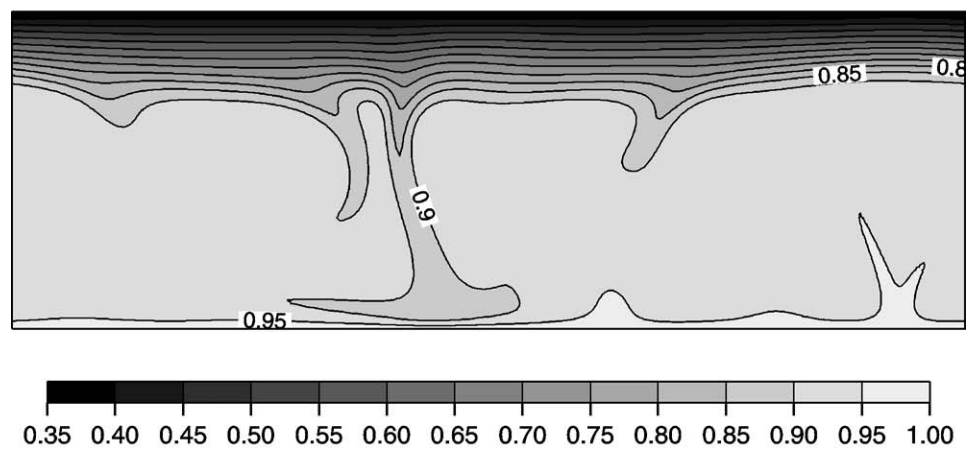
\includegraphics[width = 0.6\textwidth]{figures/LAMC/2layer}
	\caption{The internal temperature profile of the Europan ice sheet based on simulations. The color scale is temperature divided by melting temperature. Adapted from \cite{article:barr2014a}}
	\label{fig:2layer}
\end{figure}

\noindent 
\citet{article:barr2014a} examine how the combined effects conduction and convection might lead to the surface features witnessed on Europa. Based on simulations from \citet{article:showman2005a} they argue that it is likely that the ice sheet is divided up into two distinct layers: An outer layer consisting of very cold ice that is dominated by conduction, and an inner layer that is considerably warmer with convection being the key factor in the transportation of heat. The simulations indicate that the outer layer should be very thin making up only about one third of the total thickness as can be seen in Figure \ref{fig:2layer}. \\

\noindent
Other researches have come to the same conclusion, indicating that this is a likely scenario\cite{article:mckinnon1999a}\cite{article:tobie2003a}. However, \citet{article:mccarthy2016a} states that the tidal energy dissipation might be significantly higher than what has been used in previous simulations. This means that the simulation results might not represent reality after all. Because of this, both the simple linear model as well as the multilayer model will be used in the further analysis of the mission.
